\documentclass{standalone}
\usepackage{tikz}
\begin{document}
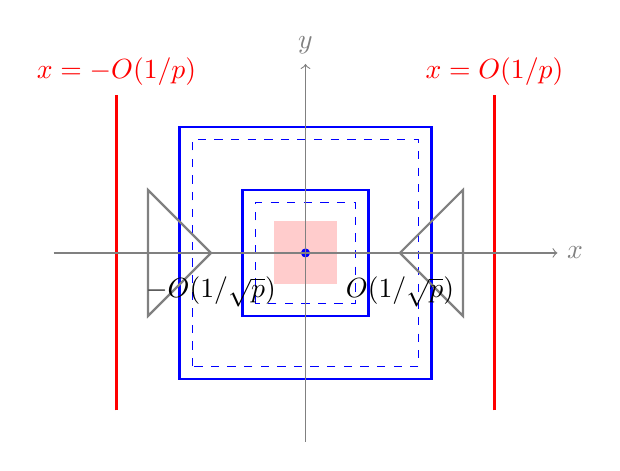
\begin{tikzpicture}[scale=0.8]
    % Red shaded area (initial confinement)
    \fill[red!20] (-0.5, -0.5) rectangle (0.5, 0.5);
    
    % First blue layer
    \draw[blue, thick] (-1, -1) rectangle (1, 1);
    \draw[dashed, blue] (-0.8, -0.8) rectangle (0.8, 0.8);
    \fill[blue] (0,0) circle (2pt);
    \draw[blue, thick] (-1, 0) -- (1, 0); % Horizontal blocking line
    
    % Second blue layer
    \draw[blue, thick] (-2, -2) rectangle (2, 2);
    \draw[dashed, blue] (-1.8, -1.8) rectangle (1.8, 1.8);
    \fill[blue] (0,0) circle (2pt);
    \draw[blue, thick] (-2, 0) -- (2, 0); % Horizontal blocking line
    
    % Vertical red lines at O(1/p) from y-axis
    \draw[red, thick] (3, -2.5) -- (3, 2.5) node[above] {$x = O(1/p)$};
    \draw[red, thick] (-3, -2.5) -- (-3, 2.5) node[above] {$x = -O(1/p)$};
    
    % Cones with vertices at O(1/√p) from x-axis
    \draw[gray, thick] (1.5, 0) -- (2.5, 1) -- (2.5, -1) -- cycle;
    \draw[gray, thick] (-1.5, 0) -- (-2.5, 1) -- (-2.5, -1) -- cycle;
    \node at (1.5, 0) [below=5pt] {$O(1/\sqrt{p})$};
    \node at (-1.5, 0) [below=5pt] {$-O(1/\sqrt{p})$};
    
    % Axes for reference (optional)
    \draw[->, gray] (-4, 0) -- (4, 0) node[right] {$x$};
    \draw[->, gray] (0, -3) -- (0, 3) node[above] {$y$};
\end{tikzpicture}
\end{document}